\section{Introduction}
\label{sec:intro}

\paragraph{The output-preconditioning dilemma.}
\mname{Muon} maps matrix momentum toward a semi-orthogonal update using Newton--Schulz iterations~\citep{jordan2024muon}, and \mname{MuonT} (also called Toner) lowers Transformer pretraining loss by preconditioning this update on the right with inverse powers of input activation second moments~\citep{mohamadi2026toner}. For a linear projection $y=Wx$, however, the backpropagated gradient $G=\sum_j\delta_jx_j^{\Tr}$ depends on both the forward activation $x_j$ and the output cotangent $\delta_j=\partial\ell/\partial y_j$. Input-only preconditioning leaves the left-hand signal unused. Extending \mname{MuonT} to the output side runs into a direct systems and quality bottleneck: computing dense spectral roots at every output (\mname{Muon2-Dense}) adds heavy cubic eigendecompositions at the end of backpropagation, whereas replacing all output roots with diagonal coordinate scaling (\mname{Muon2-Diag}) brings almost no held-out benefit and falls behind \mname{MuonT} out of distribution on wider models.

\paragraph{Structure-aware and lagged output preconditioning.}
We introduce \mname{Muon2-ExpDiag}, a structure-aware two-sided preconditioned Muon optimizer that matches output approximations and scheduling to Transformer projection role (\Cref{sec:method}). \mname{Muon2-ExpDiag} keeps \mname{MuonT}'s dense input factors and right-only weight-decay rule, applies dense $(-1/2,-1/8)$ spectral output roots to the five hidden-width projections ($\dm$: \texttt{q,k,v,o,down}), and applies exact per-step diagonal scaling to the two gated SwiGLU expansion projections ($\dff=4\dm$: \texttt{gate,up}). Because output cotangents finish arriving only at the end of backpropagation, each parameter update uses the previous step's dense output roots ($\tau=1$) while a background CUDA stream reduces current output statistics and refreshes inverse roots alongside the next step's forward and backward passes. Diagonalizing the two expansion outputs removes 96.2\% of nominal cubic output eigendecomposition work, and one-step overlap hides most of the remaining post-backward latency.

\begin{figure}[t]
  \centering
  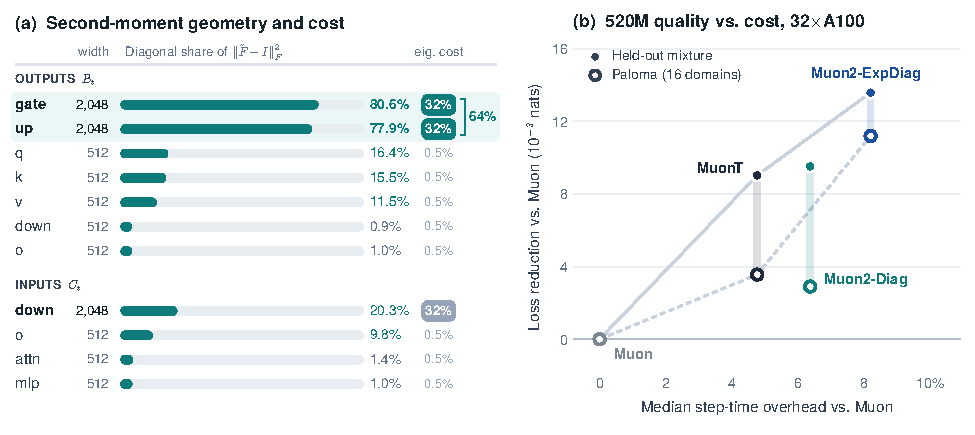
\includegraphics[width=\textwidth]{fig1_overview.pdf}
  \caption{\textbf{\mname{Muon2-ExpDiag} allocates dense output preconditioning where cross-channel geometry concentrates.}
  \textbf{(a)} Diagonal and off-diagonal shares of anisotropy across all 11 block second moments (130M, \mname{Muon} trajectory, step 2,500; 32-layer medians of $\mathrm{DiagAniso}$ in \cref{eq:diag_aniso} and $1-\mathrm{DiagAniso}$). The split shows where departure from isotropy lies in the coordinate basis rather than its total magnitude. The cost column gives each moment's share of nominal two-sided dense eigendecomposition work; teal marks the two expanded outputs (\texttt{gate,up}) that \mname{Muon2-ExpDiag} diagonalizes, which account for 96.2\% of output-side cubic work while carrying mostly diagonal anisotropy. The equally wide \texttt{down} input remains cross-channel correlated and stays dense.
  \textbf{(b)} Final held-out mixture and 16-domain Paloma loss reductions versus \mname{Muon} at 520M against median step-time overhead on 32 A100 GPUs (one seed). \mname{Muon2-ExpDiag} extends \mname{MuonT}'s quality gain with modest median overhead, whereas all-diagonal output scaling (\mname{Muon2-Diag}) adds almost no held-out gain and falls behind \mname{MuonT} on Paloma.}
  \label{fig:overview}
\end{figure}

\paragraph{Why Transformer geometry favors asymmetric compute.}
Auditing second-moment trajectories across all 32 Transformer blocks explains why \mname{Muon2-ExpDiag} allocates compute unevenly across roles and sides (\Cref{sec:diagnosis}; \Cref{fig:overview}(a)). On the gated \texttt{gate} and \texttt{up} expansion outputs, unequal coordinate second moments account for 78--91\% of total departure from isotropy, so diagonal scaling closely tracks the dense inverse root right where cubic cost concentrates. The hidden-width residual writers (\texttt{o} and \texttt{down}) show the opposite geometry: their coordinate second moments are nearly uniform, and over 99\% of their anisotropy lies in cross-channel correlations where diagonal scaling acts nearly as identity. Matrix width alone does not explain this split, because the equally wide \texttt{down} \emph{input} remains strongly correlated across channels and therefore stays dense. Over time, leading cotangent eigenspaces also rotate roughly an order of magnitude faster than RMSNormed inputs, causing cached-eigenbasis solvers to trigger frequent exact eigendecompositions that would stall synchronous updates.

\paragraph{Pretraining gains across seeds, horizon, and width.}
Across pretraining benchmarks (\Cref{sec:scaling}), \mname{Muon2-ExpDiag} improves consistently over tuned \mname{MuonT} at their shared full-budget learning rate. It lowers final held-out mixture loss by $0.0035\pm0.0017$ nats across three fresh paired seeds at 130M, by $0.0040$ nats when training four times longer (10.74B tokens), and by $0.0046$ nats under width transfer to 520M, where it also improves every one of the 16 out-of-distribution Paloma domains (\Cref{fig:overview}(b)). Across these three regimes, \mname{Muon2-ExpDiag} extends \mname{MuonT}'s held-out improvement over \mname{Muon} by 29--51\%.

\paragraph{Controls, weight decay, and update mechanism.}
Matched execution-path identity controls (\mname{Null-Ctrl}), full-budget learning-rate brackets, factor-placement ablations, and controlled comparisons with recent two-sided polar baselines (\mname{GO-MUON}, \mname{Mousse}) verify that these gains come from dense hidden-width output factors around the polar map rather than numerical drift or learning-rate mistuning (\Cref{sec:controls_ablations}). A multi-seed regularizer study further shows that keeping right-only weight decay ($W\hat R^2$) outperforms both isotropic ($W$) and two-sided ($\hat L^2 W\hat R^2$) decay across held-out, C4, and Paloma evaluations. On saved checkpoints, counterfactual probes and multi-checkpoint audits show that dense output factors rotate residual updates without inflating step norms and lower leading cotangent-subspace drift by 17--21\% relative to \mname{Muon} (\Cref{sec:mechanism_cost}).

\paragraph{Scope and runtime cost.}
Our experiments study pre-RMSNorm SwiGLU Transformers up to 537M non-embedding parameters. Relative to \mname{Muon}, expansion-output diagonalization and one-step lag cut median step-time overhead from 23.3\% (\mname{Muon2-Dense}) to 6.8\% at 130M and 8.2\% at 520M (5.3\% and 3.3\% above \mname{MuonT}), while periodic eigenbasis repairs leave mean overheads of 10.7\% and 17.0\% (8.9\% and 11.4\% above \mname{MuonT}). These results establish a fixed-token quality improvement at a modest remaining throughput cost; because the 80-TPP and 520M runs each use a single seed, multi-seed runs at larger scales are a natural next step.
